\documentclass{beamer}
\usepackage[utf8]{inputenc}

\usetheme{Madrid}
\usecolortheme{default}
\usepackage{amsmath,amssymb,amsfonts,amsthm}
\usepackage{txfonts}
\usepackage{tkz-euclide}
\usepackage{listings}
\usepackage{adjustbox}
\usepackage{array}
\usepackage{tabularx}
\usepackage{gvv}
\usepackage{lmodern}
\usepackage{circuitikz}
\usepackage{tikz}
\usepackage{graphicx}
\usepackage{gensymb} % For using \degree symbol
\usepackage{enumitem}

\setbeamertemplate{page number in head/foot}[totalframenumber]

% Title Information
\title{4.5.5}
\date{October 4, 2025}
\author{ADHARVAN KSHATHRIYA BOMMAGANI - EE25BTECH11003}

\begin{document}

% Title Slide
\frame{\titlepage}

% Question Slide
\begin{frame}{Question}
Find the vector equation of the line which is parallel to the vector $3\hat{i} - 2\hat{j} + 6\hat{k}$ and passes through the point $(1, -2, 3)$.
\end{frame}

% Step 1: General Formula
\begin{frame}{Theoretical Solution}
The vector equation of a line is given by the formula:
$$ \vec{x} = \vec{h} + t\vec{m} $$
where:
\begin{itemize}
    \item \textbf{$\vec{x}$} is the position vector of any point on the line, e.g., $\myvec{x \\ y \\ z}$.
    \bigskip
    \item \textbf{$\vec{h}$} is the position vector of a known point on the line.
    \bigskip
    \item \textbf{$\vec{m}$} is the direction vector of the line.
    \bigskip
    \item \textbf{$t$} is a scalar parameter.
\end{itemize}
\end{frame}

% Step 2: Identifying the Vectors
\begin{frame}{Theoretical Solution}
From the problem statement, we identify the components:
\bigskip
The line passes through the point $(1, -2, 3)$, so the position vector \textbf{$\vec{h}$} is:
\begin{align*}
\vec{h} = \myvec{1 \\ -2 \\ 3}
\end{align*}
\bigskip
The line is parallel to the vector $3\hat{i} - 2\hat{j} + 6\hat{k}$, so the direction vector \textbf{$\vec{m}$} is:
\begin{align*}
\vec{m} = \myvec{3 \\ -2 \\ 6}
\end{align*}
\end{frame}

% Step 3: Final Equation
\begin{frame}{Theoretical Solution}
Substituting $\vec{h}$ and $\vec{m}$ into the general equation $\vec{x} = \vec{h} + t\vec{m}$, we get the final answer.
\bigskip
\textbf{The vector equation of the line is:}
\begin{align*}
\myvec{x \\ y \\ z} = \myvec{1 \\ -2 \\ 3} + t \myvec{3 \\ -2 \\ 6}
\end{align*}
\end{frame}

% Step 4: Figure
\begin{frame}{Plot}
\centering
\textbf{Plot of the Line:}
\begin{figure}[h!]
    \centering
    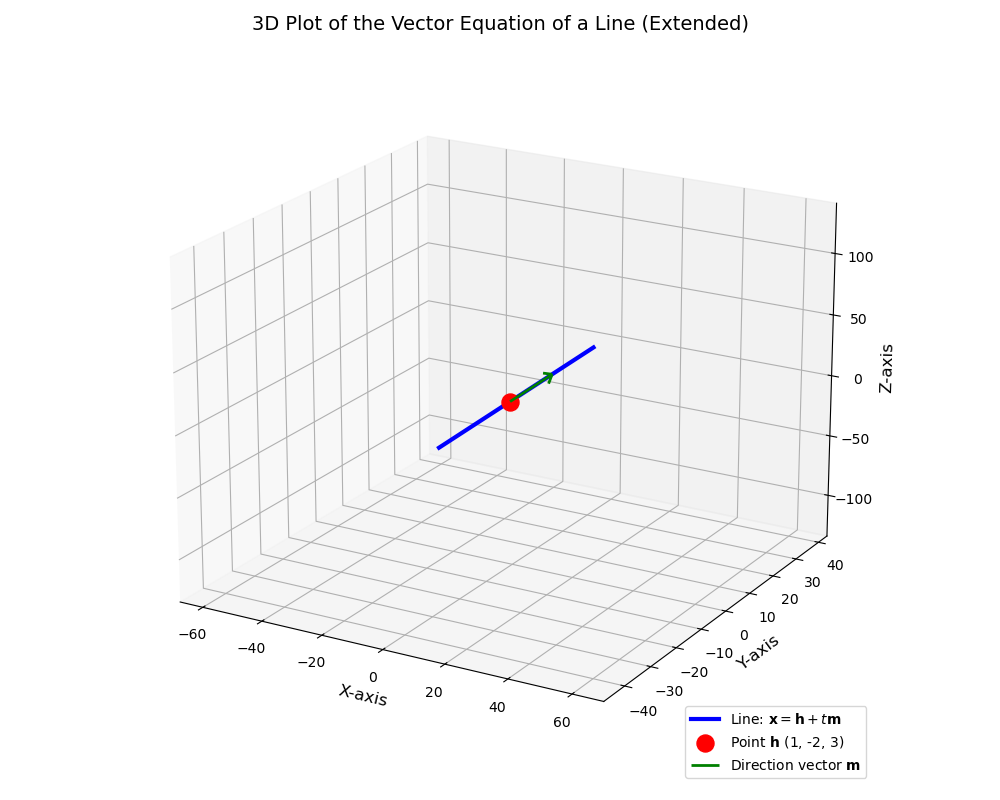
\includegraphics[width=0.8\columnwidth]{figs/fig1.png}
    \caption{3D plot showing the line, the point $\vec{h}$ (red), and the direction vector $\vec{m}$ (green).}
\end{figure}
\end{frame}

\end{document}